\ifx\allfiles\undefined
\documentclass[12pt, a4paper, oneside, UTF8]{ctexbook}
\def\path{../../config}
\usepackage{amsmath}
\usepackage{amsthm}
\usepackage{amssymb}
\usepackage{array}
\usepackage{xcolor}
\usepackage{graphicx}
\usepackage{mathrsfs}
\usepackage{enumitem}
\usepackage{geometry}
\usepackage[colorlinks, linkcolor=black]{hyperref}
\usepackage{stackengine}
\usepackage{yhmath}
\usepackage{extarrows}
\usepackage{tikz}
\usepackage{pgfplots}
\usepackage{asymptote}
\usepackage{float}
\usepackage{fontspec} % 使用字体

\setmainfont{Times New Roman}
\setCJKmainfont{LXGWWenKai-Light}[
    SlantedFont=*
]

\everymath{\displaystyle}

\usepgfplotslibrary{polar}
\usepackage{subcaption}
\usetikzlibrary{decorations.pathreplacing, positioning}

\usepgfplotslibrary{fillbetween}
\pgfplotsset{compat=1.18}
% \usepackage{unicode-math}
\usepackage{esint}
\usepackage[most]{tcolorbox}

\usepackage{fancyhdr}
\usepackage[dvipsnames, svgnames]{xcolor}
\usepackage{listings}

\definecolor{mygreen}{rgb}{0,0.6,0}
\definecolor{mygray}{rgb}{0.5,0.5,0.5}
\definecolor{mymauve}{rgb}{0.58,0,0.82}
\definecolor{NavyBlue}{RGB}{0,0,128}
\definecolor{Rhodamine}{RGB}{255,0,255}
\definecolor{PineGreen}{RGB}{0,128,0}

\graphicspath{ {figures/},{../figures/}, {config/}, {../config/} }

\linespread{1.6}

\geometry{
    top=25.4mm, 
    bottom=25.4mm, 
    left=20mm, 
    right=20mm, 
    headheight=2.17cm, 
    headsep=4mm, 
    footskip=12mm
}

\setenumerate[1]{itemsep=5pt,partopsep=0pt,parsep=\parskip,topsep=5pt}
\setitemize[1]{itemsep=5pt,partopsep=0pt,parsep=\parskip,topsep=5pt}
\setdescription{itemsep=5pt,partopsep=0pt,parsep=\parskip,topsep=5pt}

\lstset{
    language=Mathematica,
    basicstyle=\tt,
    breaklines=true,
    keywordstyle=\bfseries\color{NavyBlue}, 
    emphstyle=\bfseries\color{Rhodamine},
    commentstyle=\itshape\color{black!50!white}, 
    stringstyle=\bfseries\color{PineGreen!90!black},
    columns=flexible,
    numbers=left,
    numberstyle=\footnotesize,
    frame=tb,
    breakatwhitespace=false,
} 

\lstset{
    language=TeX, % 设置语言为 TeX
    basicstyle=\ttfamily, % 使用等宽字体
    breaklines=true, % 自动换行
    keywordstyle=\bfseries\color{NavyBlue}, % 关键字样式
    emphstyle=\bfseries\color{Rhodamine}, % 强调样式
    commentstyle=\itshape\color{black!50!white}, % 注释样式
    stringstyle=\bfseries\color{PineGreen!90!black}, % 字符串样式
    columns=flexible, % 列的灵活性
    numbers=left, % 行号在左侧
    numberstyle=\footnotesize, % 行号字体大小
    frame=tb, % 顶部和底部边框
    breakatwhitespace=false % 不在空白处断行
}

% \begin{lstlisting}[language=TeX] ... \end{lstlisting}

% 定理环境设置
\usepackage[strict]{changepage} 
\usepackage{framed}

\definecolor{greenshade}{rgb}{0.90,1,0.92}
\definecolor{redshade}{rgb}{1.00,0.88,0.88}
\definecolor{brownshade}{rgb}{0.99,0.95,0.9}
\definecolor{lilacshade}{rgb}{0.95,0.93,0.98}
\definecolor{orangeshade}{rgb}{1.00,0.88,0.82}
\definecolor{lightblueshade}{rgb}{0.8,0.92,1}
\definecolor{purple}{rgb}{0.81,0.85,1}

\theoremstyle{definition}
\newtheorem{myDefn}{\indent Definition}[section]
\newtheorem{myLemma}{\indent Lemma}[section]
\newtheorem{myThm}[myLemma]{\indent Theorem}
\newtheorem{myCorollary}[myLemma]{\indent Corollary}
\newtheorem{myCriterion}[myLemma]{\indent Criterion}
\newtheorem*{myRemark}{\indent Remark}
\newtheorem{myProposition}{\indent Proposition}[section]

\newenvironment{formal}[2][]{%
	\def\FrameCommand{%
		\hspace{1pt}%
		{\color{#1}\vrule width 2pt}%
		{\color{#2}\vrule width 4pt}%
		\colorbox{#2}%
	}%
	\MakeFramed{\advance\hsize-\width\FrameRestore}%
	\noindent\hspace{-4.55pt}%
	\begin{adjustwidth}{}{7pt}\vspace{2pt}\vspace{2pt}}{%
		\vspace{2pt}\end{adjustwidth}\endMakeFramed%
}

\newenvironment{definition}{\vspace{-\baselineskip * 2 / 3}%
	\begin{formal}[Green]{greenshade}\vspace{-\baselineskip * 4 / 5}\begin{myDefn}}
	{\end{myDefn}\end{formal}\vspace{-\baselineskip * 2 / 3}}

\newenvironment{theorem}{\vspace{-\baselineskip * 2 / 3}%
	\begin{formal}[LightSkyBlue]{lightblueshade}\vspace{-\baselineskip * 4 / 5}\begin{myThm}}%
	{\end{myThm}\end{formal}\vspace{-\baselineskip * 2 / 3}}

\newenvironment{lemma}{\vspace{-\baselineskip * 2 / 3}%
	\begin{formal}[Plum]{lilacshade}\vspace{-\baselineskip * 4 / 5}\begin{myLemma}}%
	{\end{myLemma}\end{formal}\vspace{-\baselineskip * 2 / 3}}

\newenvironment{corollary}{\vspace{-\baselineskip * 2 / 3}%
	\begin{formal}[BurlyWood]{brownshade}\vspace{-\baselineskip * 4 / 5}\begin{myCorollary}}%
	{\end{myCorollary}\end{formal}\vspace{-\baselineskip * 2 / 3}}

\newenvironment{criterion}{\vspace{-\baselineskip * 2 / 3}%
	\begin{formal}[DarkOrange]{orangeshade}\vspace{-\baselineskip * 4 / 5}\begin{myCriterion}}%
	{\end{myCriterion}\end{formal}\vspace{-\baselineskip * 2 / 3}}
	

\newenvironment{remark}{\vspace{-\baselineskip * 2 / 3}%
	\begin{formal}[LightCoral]{redshade}\vspace{-\baselineskip * 4 / 5}\begin{myRemark}}%
	{\end{myRemark}\end{formal}\vspace{-\baselineskip * 2 / 3}}

\newenvironment{proposition}{\vspace{-\baselineskip * 2 / 3}%
	\begin{formal}[RoyalPurple]{purple}\vspace{-\baselineskip * 4 / 5}\begin{myProposition}}%
	{\end{myProposition}\end{formal}\vspace{-\baselineskip * 2 / 3}}


\newtheorem{example}{\indent \color{SeaGreen}{Example}}[section]
\renewcommand{\proofname}{\indent\textbf{\textcolor{TealBlue}{Proof}}}
\NewEnviron{solution}{%
	\begin{proof}[\indent\textbf{\textcolor{TealBlue}{Solution}}]%
		\color{blue}% 设置内容为蓝色
		\BODY% 插入环境内容
		\color{black}% 恢复默认颜色(可选,避免影响后续文字)
	\end{proof}%
}

% 自定义命令的文件

\def\d{\mathrm{d}}
\def\R{\mathbb{R}}
%\newcommand{\bs}[1]{\boldsymbol{#1}}
%\newcommand{\ora}[1]{\overrightarrow{#1}}
\newcommand{\myspace}[1]{\par\vspace{#1\baselineskip}}
\newcommand{\xrowht}[2][0]{\addstackgap[.5\dimexpr#2\relax]{\vphantom{#1}}}
\newenvironment{mycases}[1][1]{\linespread{#1} \selectfont \begin{cases}}{\end{cases}}
\newenvironment{myvmatrix}[1][1]{\linespread{#1} \selectfont \begin{vmatrix}}{\end{vmatrix}}
\newcommand{\tabincell}[2]{\begin{tabular}{@{}#1@{}}#2\end{tabular}}
\newcommand{\pll}{\kern 0.56em/\kern -0.8em /\kern 0.56em}
\newcommand{\dive}[1][F]{\mathrm{div}\;\boldsymbol{#1}}
\newcommand{\rotn}[1][A]{\mathrm{rot}\;\boldsymbol{#1}}

\newif\ifshowanswers
\showanswerstrue % 注释掉这行就不显示答案

% 定义答案环境
\newcommand{\answer}[1]{%
    \ifshowanswers
        #1%
    \fi
}

% 修改参数改变封面样式,0 默认原始封面、内置其他1、2、3种封面样式
\def\myIndex{0}


\ifnum\myIndex>0
    \input{\path/cover_package_\myIndex} 
\fi

\def\myTitle{考研数学笔记}
\def\myAuthor{Weary Bird}
\def\myDateCover{\today}
\def\myDateForeword{\today}
\def\myForeword{相见欢·林花谢了春红}
\def\myForewordText{
    林花谢了春红,太匆匆。
    无奈朝来寒雨晚来风。
    胭脂泪,相留醉,几时重。
    自是人生长恨水长东。
}
\def\mySubheading{以姜晓千强化课讲义为底本}


\begin{document}
\else
\fi

\chapter{一元函数积分学}
\section{ 定积分的概念}

\begin{enumerate}[label=\arabic*.,start=2]
    \item (2009,数三)使不等式$\int_1^x\frac{\sin t}{t} dt>\ln x$成立的$x$的范围是 \\
        $(A)\ (0,1)\quad(B)\left(1,\frac{\pi}{2}\right)\quad
        (C)\left(\frac{\pi}{2},\pi\right)\quad(D)(\pi,+\infty)$
    
    \begin{solution}
    (方法一) 利用单调性
    \begin{align*}
        f(x)  &= \int_{1}^{x}\frac{\sin{t}}{t}\d t -\ln{x} \\
        f'(x) &= \frac{\sin{x} - 1}{x}\begin{cases}
            x > 0 &, f'(x) < 0 \\
            x < 0 &, f'(x) > 0
        \end{cases}
    \end{align*}
    又$f(1)=0$故$f(x)$在$(0,1)$上大于0,在$(1,\infty)$小于0 \\
    (方法二) 利用几何意义 
    \begin{align*}
        &\int_{1}^{x}\frac{\sin t}{t}\d t > \ln{x} = \int_{1}^{x}\frac{1}{t}\d t \\
        &\int_{1}^{x}\frac{\sin{t} - 1}{t}\d t > 0
    \end{align*}
    由积分的几何意义容易知道,当$x\in(0,1)$时候上式成立
    \end{solution}
    
    \item (2003,数二)设$I_1=\int_0^{\frac{\pi}{4}}\frac{\tan x}{x} dx, 
    I_2=\int_0^{\frac{\pi}{4}}\frac{x}{\tan x} dx$,则 \\
    (A) $I_1>I_2>1$\quad(B) $1>I_1>I_2$ \\
    (C) $I_2>I_1>1$\quad(D) $1>I_2>I_1$
    
    \begin{solution}
    由基本不等式$x\in(0,\frac{\pi}{2}),\sin{x}<x<\tan{x}$,故有$\tan{x}/x > 1 > x/\tan{x}$ 
    由比较定理有$I_1>I_1$,考虑$I_1$与$1$的关系. \\
    (方法一) 求导用单调性 \\
    $f(x)=\tan{x}/x$ ,则
    \begin{align*}
        f'(x) &=\frac{\sec^2{x}\cdot x-\tan{x}}{x^2} \\
        &= \frac{x-\sin{x}\cos{x}}{\cos^2{x}x^2} > 0
    \end{align*}
    故$f(x)$在$(0,\pi/4)$上单调递增,有$f(x)<f(\pi/4)=\frac{4}{\pi}$,故$I_1<1$ \\
    (方法二) 利用凹凸性 \\
    由于$\tan{x}$在$(0,\pi/2)$上是一个凹函数,则其割线的函数值大于函数的函数值大于切线的函数值(割线在函数图像的上方,切线
    在函数图像的下方)则有
    $$
    \frac{4}{\pi} > \tan{x}
    $$
    从而$I_1<1$
    \end{solution}
\end{enumerate}

\section{ 不定积分的计算}
\begin{remark}
    $$
    \text{不定积分的计算}
    \begin{cases}
        \text{凑微分} \\
        \text{分部} \\
        \text{换元} \begin{cases}
            \text{倒代换} \\
            \text{三角代换} \\
            \text{根式代换} \\
            \text{万能公式} \\
            \text{整体代换}
        \end{cases}
    \end{cases}
    $$
分部里面要注意表格积分法,与行列式积分法 \\`'
万能公式如下
\begin{align*}
    \text{令}t=\tan{\frac{x}{2}}\text{则}
    \begin{cases}
        \sin{x}=\frac{2t}{1+t^2} \\
        \cos{x}=\frac{1-t^2}{1+t^2} \\
        \tan{x}=\frac{\sin{x}}{\cos{x}}=\frac{1-t^2}{2t}\\
        x=2\cdot\arctan{t}, \d x = \frac{2}{1+t^2}\d t
    \end{cases}
\end{align*}
\end{remark}

\begin{enumerate}[label=\arabic*.,start=4]
    \item 计算下列积分(1)$\int\frac{x^2+1}{x^4+1}\d x$;(2)$\int\frac{x^2-1}{x^4+1}\d x$
    
    \begin{solution}
    (1) 
    \begin{align*}
        \text{原式} &= \int\frac{1+\frac{1}{x^2}}{x^2+\frac{1}{x^2}}\d x \\
        &= \int\frac{\d (x-\frac{1}{x})}{(x-\frac{1}{x})^2 + 2} \\
        &\xlongequal{\int\frac{1}{x^2+a^2}\d x}\frac{1}{\sqrt{2}}\arctan{\frac{x-\frac{1}{x}}{\sqrt{2}}} + C
    \end{align*}
    (2) 
    \begin{align*}
        \text{原式} &= \int\frac{1 - \frac{1}{x^2}}{x^2+\frac{1}{x^2}} \\
        &= \int\frac{\d (x+\frac{1}{x})}{(x+\frac{1}{x})^2 - 2} \\
        &\xlongequal{\int\frac{1}{a^2-x^2}\d x}-\frac{1}{2\sqrt{2}}\ln\left|{\frac{\sqrt{2}+(x+\frac{1}{x})}{\sqrt{2}-(x+\frac{1}{x})}}\right|
    \end{align*}
    \end{solution}
    
    \item 计算不定积分$\int\ln\left(1+\sqrt{\frac{1+x}{x}}\right)\d x, x>0$
    
    \begin{solution}
        \begin{align*}
        \text{原式} &\xlongequal{t=\sqrt\frac{(1+x)}{x}}\ln{1+t}\d (\frac{1}{t^2 - 1}) \\
        &\xlongequal{\text{分部积分}}\ln{(1+t)}\cdot\frac{1}{t^2-1}-\int\frac{1}{t^2-1}\cdot\frac{1}{1+t}\d t \\
        \int\frac{1}{t^2-1}\cdot\frac{1}{1+t}\d t &=\frac{1}{2}\int\frac{\d t}{t^2 - 1} - \frac{1}{2}\int\frac{\d t}{(t+1)^2} \\
        &=-\frac{1}{4}\ln\left|\frac{1+t}{1-t}\right| + \frac{1}{2(1+t)} + C \\
        \text{原式} &= \ln{(1+t)}\cdot\frac{1}{t^2-1} + \frac{1}{4}\ln\left|\frac{1+t}{1-t}\right| + \frac{1}{2(1+t)} + C 
    \end{align*}
    \end{solution}

    \item  求$\int\frac{1}{1+\sin x+\cos x} dx$
    
    \begin{solution}
    (方法一\ 万能代换)
    \begin{align*}
        \text{原式} &\xlongequal{t=\tan{\frac{x}{2}}} \int\frac{\d t}{1+t} \\
        &=\ln\left|1+t\right| + C \\
        &=\ln\left|1+\tan{\frac{x}{2}}\right| + C
    \end{align*}
    (方法二\ 三角公式) 
    \begin{align*}
        \text{原式}&\xlongequal{\cos{x}=2\cos^2{\frac{x}{2}}-1}\int\frac{\d x}{2\cos^2{\frac{x}{2}}+2\sin{\frac{x}{2}}\cos{\frac{x}{2}}} \\
        &=\int\frac{\d x}{2\cos^2{\frac{x}{2}}(1+\tan{x}{2})} \\
        &=\int\frac{\d \tan{\frac{x}{2}}}{1+\tan\frac{x}{2}} \\
        &=\ln\left|1+\tan{\frac{x}{2}}\right| + C
    \end{align*}
    \end{solution}
\end{enumerate}

\section{定积分的计算}
\begin{remark}
    定积分除了不定积分的办法还有如下自己独有的办法
    $$
        \text{定积分的计算}\begin{cases}
            \text{奇偶性} \\
            \text{周期性} \\
            \text{华里士公式} \\
            \text{区间再现}
        \end{cases}
    $$
    其中华里士公式如下 
    $$
    \int_{0}^{\frac{\pi}{2}}\sin^{n}{x}\d x\begin{cases}
        \frac{n-1}{n}\cdot\frac{n-3}{n-2}\ldots\frac{2}{3}\cdot 1, & n=\text{奇数} \\
        \frac{n-1}{n}\cdot\frac{n-3}{n-2}\ldots\frac{1}{2}\cdot\frac{\pi}{2}, & n=\text{偶数}
    \end{cases}
    $$
    $\cos{x}$也是一样的结果
\end{remark}
\begin{enumerate}[label=\arabic*.,start=7]
    \item (2013,数一)计算$\int_0^1\frac{f(x)}{\sqrt{x}} dx$,其中$f(x)=\int_1^x\frac{\ln(t+1)}{t} dt$
    
    \begin{solution}
    (方法一\ 分部积分法) 
    \begin{align*}
        \text{原式} &=2\int_{0}^{1}f(x)\d \sqrt{x} \\
        &= -2\int_{0}^{1}\frac{\ln{(1+x)}}{\sqrt{x}}\d x \\
        &\xlongequal{\sqrt{x}=t}-4\int_{0}^{1}\ln{(1+t^2)}\d t \\
        &=-4t\ln{(1+t^2)}\bigg|_{0}^{1}+4\int_{0}^{1}\frac{2t^2}{t^2+1}\d t \\
        &= 8 -4\ln{2}-2\pi 
    \end{align*}
    (方法二\ 二重积分) 
    \begin{align*}
        \text{原式} &=\int_{0}^{1}\frac{1}{\sqrt{x}}\d x\int_{1}^{x}\frac{\ln{(1+t)}}{t}\d t \\
        &\xlongequal{\text{交换积分次序}}-\int_{0}^{1}\frac{\ln{(1+t)}}{t}\d t\int_{0}^{t}\frac{1}{\sqrt{x}}\d x \\
        &=-2\int_{0}^{1}\frac{\ln{(1+t)}}{\sqrt{t}}\d t \\
        &=\ldots \\
        &=8 -4\ln{2}-2\pi 
    \end{align*}
    \end{solution}
    
    \item  求下列积分:
    $
        (1)\ \int_{0}^{\frac{\pi}{2}}\frac{e^{sin x}}{e^{sin x}+e^{cos x}}\d x \\
        (2)\ \int_0^{\frac{\pi}{2}}\frac{1}{1+(\tan x)^{\sqrt{2}}} dx
    $
    \begin{solution}
    这两题都是典型的区间再现的题目 \\
    (1)
    \begin{align*}
        \text{原式}\xlongequal{x=\frac{\pi}{2}-t}\int_{0}^{\frac{\pi}{2}}\frac{e^{\cos{t}}}{e^{\sin{t}}+e^{\cos{t}}}\d t 
    \end{align*}
    由于积分与变量无关,将上式与原式相加有 
    $$
    \text{原式}=\frac{1}{2}\int_{0}^{\frac{\pi}{2}}\d t = \frac{\pi}{4}
    $$
    (2) 
    \begin{align*}
        \text{原式} &=\int_{0}^{\frac{\pi}{2}}\frac{(\cos{x})^{\sqrt{2}}}{(\sin{x})^{\sqrt{2}}+\cos{x})^{\sqrt{2}}} \\
        &\xlongequal{\text{和一完全一致}}\ldots \\
        &=\frac{\pi}{4}
    \end{align*}
    \end{solution}
    \item  求$\int_0^{\frac{\pi}{4}}\ln(1+\tan x) dx$
    
    \begin{solution}
    这道题是比较困难的积分计算题,由于其他方法都不好用不妨考虑区间再现
    \begin{align*}
        \text{原式}&\xlongequal{x=\frac{\pi}{4}-t}=\int_{0}^{\frac{\pi}{4}}\ln{\left[1+\tan{(\frac{\pi}{4}-t)}\right]}\d t \\
        &\xlongequal{\tan{(a+b)}=\frac{\tan{a}+\tan{b}}{1-\tan{a}\tan{b}}}\int_{0}^{\frac{\pi}{4}}\left[\ln{2}-\ln{(1+\tan{t})}\right]\d t \\
        \text{原式} &=\frac{\pi}{8}\ln{2}
    \end{align*}
    \end{solution}

    \begin{tcolorbox}[title=区间再现总结]
        考试中可能直接考察的区间再现的公式为 
        $$
        \int_{0}^{\pi}xf(\sin{x})\d x = \frac{\pi}{2}\int_{0}^{\pi}f(\sin x)\d x
        $$
        其余的就只能\underline{见机行事}若其他积分方法都无法做出则可以考虑区间再现
    \end{tcolorbox}
\end{enumerate}

\section{ 反常积分的计算}
\begin{remark}
    瑕积分的计算需要注意,若瑕点在内部则需要积分拆开分别计算
\end{remark}

\begin{enumerate}[label=\arabic*.,start=10]
    \item (1998,数二)计算积分$\int_{\frac{1}{2}}^{\frac{3}{2}}\frac{\d x}{\sqrt{\left|x-x^2\right|}}$
    
    \begin{solution}
    显然$x=1$是积分的瑕点,故原积分需要拆成两部分即
    \begin{align*}
        \text{原式} &=\int_{\frac{1}{2}}^{1}\frac{\d x}{\sqrt{x-x^2}}+\frac{1}{\frac{3}{2}}\frac{\d x}{\sqrt{x^2-x}} \\
        &\xlongequal{\text{配方}}\arcsin{2(x-\frac{1}{2})}\bigg|_{\frac{1}{2}}^{1}+\ln\left|x-\frac{1}{2}+\sqrt{(x-\frac{1}{2})^2-\frac{1}{4}}\right|\bigg|_{1}^{\frac{3}{2}} \\
        &=\frac{\pi}{2}+\ln\left(2+\sqrt{3}\right)
    \end{align*}
    \end{solution}

    \begin{tcolorbox}[title=积分表的拓展]
        \begin{enumerate}
            \item [(1)]
            \begin{align*}
                \int\frac{\d x}{\sqrt{a^2-x^2}} &=\arcsin\frac{x}{a}+C\\
                \int\sqrt{a^2-x^2}\d x &=\frac{x}{2}\sqrt{a^2-x^2}+\frac{a^2}{2}\arcsin\frac{x}{a}+C
            \end{align*}
            \item [(2)]
            \begin{align*}
                \int\frac{\d x}{\sqrt{x^2+a^2}} &=\ln{\left|x+\sqrt{x^2+a^2}\right|} \\
                \int\sqrt{x^2+a^2}\d x &=\frac{x}{2}\sqrt{x^2+a^2}+\frac{a^2}{2}\ln\left|x+\sqrt{x^2+a^2}\right| + C 
            \end{align*}
            \item [(3)]
            \begin{align*}
                \int\frac{\d x}{\sqrt{x^2-a^2}} &=\ln{\left|x+\sqrt{x^2 - a^2}\right|} \\
                \int\sqrt{x^2-a^2}\d x &=\frac{x}{2}\sqrt{x^2-a^2}-\frac{a^2}{2}\ln\left|x+\sqrt{x^2-a^2}\right| + C 
            \end{align*}
            第二个如果是定积分也可以按照几何意义(圆的面积)做
        \end{enumerate}
    \end{tcolorbox}
\end{enumerate}

\section{ 反常积分敛散性的判定}
\begin{remark}
    反常积分的敛散性感觉不如无穷级数敛散性难 \\
    (方法一)使用反常积分的定义,算出其极限值 \\
    (方法二)比较判别法--寻找 $x^p$ 
    \begin{align*}
        (\text{瑕积分})\int_{0}^{1}\frac{1}{x^p}\begin{cases}
            0<p<1, &\text{收敛} \\
            p\geq 1, &\text{发散}
        \end{cases} \\
        (\text{无穷积分})\int_{1}^{+\infty}\frac{1}{x^p}\begin{cases}
            p > 1, &\text{收敛} \\
            p\leq 1, &\text{发散}
        \end{cases}
    \end{align*}
\end{remark}
\newpage
\begin{enumerate}[label=\arabic*.,start=11]
    \item (2016,数一)若反常积分$\int_0^{+\infty}\frac{1}{x^a(1+x)^b} dx$收敛,则 \\
        (A)\ a<1且\ b>1 \qquad
        (B)\ a>1且\ b>1 \\
        (C)\ a<1且\ a+b>1 \qquad
        (D)\ a>1且\ a+b>1
    
    \begin{solution}
    显然$x=0$是该积分的瑕点,需要分成两部分考虑 $\int_{0}^{+\infty}=\int_{0}^{1}+\int_{1}^{+\infty}$
    \begin{align*}
        &\lim_{x\to 0^{+}}\frac{x^p}{x^{a}(1+x)^b}= {\color{red} 1} \\
        &\xlongequal{\text{等价代换}}\lim_{x\to 0^+}\frac{x^p}{x^a} \implies p = a
    \end{align*}
    由p积分的性质可知当$p<1$的时候其收敛故$a<1$的时候原积分中的$\int_{0}^{1}$收敛
    同理对于$\int_{1}^{+\infty}$有 
    \begin{align*}
        \lim_{x\to +\infty}\frac{x^p}{x^{a+b}} = 1\implies p = a + b
    \end{align*}
    由p积分的性质可知当$p>1$即$a+b>1$的时候原积分$\int_{1}^{+\infty}$收敛,故由反常积分的定义可知只有$a<1,a+b>1$的时候
    原积分收敛
    \end{solution}
    
    \item (2010,数一、数二)设$m,n$均为正整数,则反常积分$\int_0^1\frac{\sqrt[m]{\ln^2(1-x)}}{\sqrt[n]{x}} dx$的收敛性 \\
        (A)\ 仅与\ m\ 的取值有关 \qquad
        (B)\ 仅与\ n\ 的取值有关 \\
        (C)\ 与\ m,n\ 的取值都有关 \qquad
        (D)\ 与\ m,n\ 的取值都无关
    
    \begin{solution}
    显然$x=0$和$x=1$是积分的瑕点,需要分成两部分考虑,有$\int_{0}^{1}=\int_{0}^{\frac{1}{2}}+\int_{\frac{1}{2}}^{1}$,想考虑前一个积分
    \begin{align*}
        \lim_{x\to 0^+}\int_{0}^{\frac{1}{2}}x^p\frac{\sqrt[m]{\ln^{2}{(1-x)}}}{\sqrt[n]{x}} = \lim_{x\to 0^+}\int_{0}^{\frac{1}{2}}x^p\frac{1}{x^{\frac{1}{n}-\frac{2}{m}}} \implies p = \frac{1}{n}-\frac{2}{m}
    \end{align*}
    由p积分的性质,只有$p<1$上述积分就收敛,而由于$(n,m)\in\mathbb{Z}^+,\frac{1}{n}-\frac{2}{m}<\frac{1}{n}<1$ 故上式恒收敛. 
    \begin{align*}
        \lim_{x\to 1^{-}}(x-1)^p\frac{\sqrt[m]{\ln{(1-x)^2}}}{\sqrt[n]{x}} =\lim_{x\to 1^{-}}(x-1)^{p}\sqrt[m]{\ln(1-x)^2} \implies \text{恒为0}    
    \end{align*}
    故上式也恒收敛,故原式的敛散性与$(n,m)$均无关
    \end{solution}
\end{enumerate}

\section{ 变限积分函数}
\begin{tcolorbox}[title={原函数,可积,变限积分}]
    (一)原函数存在定理 
    $$
    \int f(x)\d x\text{存在}\begin{cases}
        \text{连续函数原函数必然存在} \\
        \text{含有第一类间断点和无穷间断点其原函数必然不存在}\\
        \text{含有震荡间断点其原函数可能存在} 
    \end{cases}
    $$
    (二)可积性定理 
    $$
    \int_{a}^{b}f(x)\d x\text{存在}\begin{cases}
        \text{可积必有界} \\
        \text{连续必可积} \\
        \text{含有有限个间断点的有界函数可积}
    \end{cases}
    $$
    (三)变限积分 
    $$
    F(x)=\int_{a}^{x}f(t)\d t\begin{cases}
        f(x)\text{可积}\implies F(x)\text{连续} \\
        f(x)\text{连续}\implies F(x)\text{可导} \\
        x=x_0\text{是函数可去间断点}\implies F(x)\text{可导,但},F'(x_0)\neq f(x_0) \\
        x=x_0\text{是函数跳跃间断点}\implies F(x)\text{不可导,但连续}
    \end{cases}
    $$
\end{tcolorbox}
\begin{enumerate}[label=\arabic*.,start=13]
    \item (2013,数二)设函数$f(x)=\begin{cases}
        \sin x, & 0\leq x<\pi \\
        2, & \pi\leq x\leq 2\pi
    \end{cases}$,$F(x)=\int_0^x f(t) dt$,则 \\
    (A)\ x=$\pi$\ 是函数\ F(x)\ 的跳跃间断点 \qquad
    (B)\ x=$\pi$\ 是函数\ F(x)\ 的可去间断点 \\
    (C)\ F(x)\ 在\ x=$\pi$\ 处连续但不可导 \qquad
    (D)\ F(x)\ 在\ x=$\pi$\ 处可导
    
    \begin{solution}
    显然由总结可知,选C
    \end{solution}
    
    \item (2016,数二)已知函数$f(x)$在$[0,\frac{3\pi}{2}]$上连续,在$(0,\frac{3\pi}{2})$内是函数
    $\frac{\cos{x}}{2x-3\pi}$的一个原函数,且$f(0)=0$.
    \begin{enumerate}[label=(\roman*)]
        \item[(1)] 求$f(x)$在区间$[0,\frac{3\pi}{2}]$上的平均值;
        \item[(2)] 证明$f(x)$在区间$[0,\frac{3\pi}{2}]$内存在唯一零点.
    \end{enumerate}
    
    \begin{solution}
    (一)有题有$f(x)=\int_{0}^{x}\frac{\cos{t}}{2t-3\pi}\d t$,所求的平均值为 
    \begin{align*}
        \text{平均值} &=\frac{\int_{0}^{\frac{3\pi}{2}}f(x)\d x}{\frac{3\pi}{2}} \\
        &=\frac{\int_{0}^{\frac{3\pi}{2}}\int_{0}^{x}\frac{\cos{t}}{2t-3\pi}\d t}{\frac{3\pi}{2}} \\
        &\xlongequal{\text{交换积分次序}} \frac{2}{3\pi}\int_{0}^{\frac{3\pi}{2}}\frac{\cos{t}}{2t-3\pi}\d t\int_{t}^{\frac{3\pi}{2}}\d x \\
        &=\frac{1}{3\pi}
    \end{align*}
    (二)有题可知$f'(x)=\frac{\cos{x}}{2x-3\pi}$,在$(0,\frac{3\pi}{2})$只有唯一零点$x=\frac{\pi}{2}$,从而有
    $0<x<\frac{\pi}{2},f(x)$ 单调递减,而$\frac{\pi}{2} < x < \frac{3\pi}{2}, f(x)$ 单调递增,且$f(0)=0$,考虑上述平均值,由积分中值定理有
    $f(c)=\frac{\pi}{3}>0$ 故$f(x)$在$\frac{\pi}{2}\sim\frac{3\pi}{2}$上有一个零点.综上$f(x)$在区间$(0,\frac{3\pi}{2})$仅有一个零点 
    \end{solution}
\end{enumerate}

\begin{tcolorbox}[title=定积分的应用]
    (一)定积分求面积(也可以用二重积分)
    $$
    A = 
    \begin{cases}
        \int_{a}^{b}\left|f(x)\right|\d x, &\text{直角坐标系} \\
        \frac{1}{2}\int_{\alpha}^{\beta}r^2(\theta)\d \theta, &\text{极坐标} \\
        \int_{\alpha}^{\beta}\left|y(t)x'(t)\right|\d t, &\text{参数方程} \\
        \frac{1}{2}\int_{l}-y\d x + x\d y, &\text{L对D来说取正向}
    \end{cases}
    $$
    (二)定积分求旋转体体积(可以用微元法推,也可以用二重积分)
    $$
    V = 
    \begin{cases}
        \iint_{D}2\pi r(x,y)\d \sigma, & \text{二重积分法,其中}r(x,y)\text{为区域D内一点到转轴的距离} \\
        \int_{a}^{b}\pi f^2(x)\d x, &\text{微元法,绕x轴旋转} \\
        \int_{a}^{b}2\pi\left|xf(x)\right|\d x, &\text{微元法,绕y轴旋转} 
    \end{cases}
    $$
    (三)定积分求弧长(第一类曲线积分)
    $$
    s_{\text{弧长}} = \int_{C}f(x,y)\d s = 
    \begin{cases}
        \int_{a}^{b}\d s = \int_{a}^{b}\sqrt{1+(y')^2}\d x, &\text{直角坐标} \\
        \int_{\alpha}^{\beta}\d s = \int_{\alpha}^{\beta}\sqrt{(x'(t))^2+(y'(t))^2}\d t, &\text{参数方程} \\
        \int_{\alpha}^{\beta}\d s = \int_{\alpha}^{\beta}\sqrt{r^2(\theta)+r'^2(\theta)}\d \theta, &\text{极坐标}
    \end{cases}
    $$
    (四)定积分求侧面积(第一类曲面积分)
    $$
    S_{\text{侧面积}} = \iint_{S}\d S = \begin{cases}
        \int_{a}^{b}2\pi y(x)\sqrt{1+(y'(x))^2}\d x, &\text{直角坐标} \\
        \int_{\alpha}^{\beta}2\pi y(t)\sqrt{(x'(t))^2+(y'(t))^2}\d t, &\text{参数方程} \\
        \int_{\alpha}^{\beta}2\pi r(\theta)\sin{\theta}\sqrt{r^2(\theta)+r'^2(\theta)}\d\theta, &\text{极坐标}
    \end{cases}
    $$
    (五)物理应用(微元法,不过数一不太可能考)
\end{tcolorbox}

\newpage

\section{ 定积分应用求面积}

\begin{enumerate}[label=\arabic*.,start=15]
    \item (2019,数一、数二、数三)求曲线$y=e^{-x}\sin x(x\geq 0)$与$x$轴之间图形的面积.
    
    \begin{solution}
    \begin{align*}
        A &=\int_{0}^{+\infty}\left|e^x\sin{x}\right|\d x \\
        &=\sum_{n=0}^{\infty}(-1)^n\int_{n\pi}^{(n+1)\pi}e^{-x}\sin{x}\d x \\
        \text{由于}\int e^{\alpha x}\sin{\beta x}\d x &= \frac{\begin{vmatrix}
            (e^{\alpha x})' & (\sin{\beta{x}})' \\
            e^{\alpha x} & (\sin{\beta x})
        \end{vmatrix}}{\alpha ^ 2 + \beta ^ 2} + C\\
        \text{其中}\int_{n\pi}^{(n+1)\pi}e^{-x}\sin{x}\d x &=\frac{-e^{-x}(\sin{x}+\cos{x})}{2}\bigg|^{(n+1)\pi}_{n\pi} \\
        \text{故原式} &= \frac{1}{2}\sum_{n=0}^{\infty}e^{-n\pi}(1+e^{-\pi}) \\
        &=\frac{1+e^{-\pi}}{2}\cdot\frac{1}{1-e^{-\pi}} = \frac{1+e^{\pi}}{2(e^{\pi}-1)}
    \end{align*}
    \end{solution}
\end{enumerate}

\section{ 定积分应用求体积}

\begin{enumerate}[label=\arabic*.,start=16]
    \item (2003,数一)过原点作曲线$y=\ln x$的切线,该切线与曲线$y=\ln x$及$x$轴围成平面图形$D$.
    \begin{enumerate}[label=(\roman*)]
        \item[(1)] 求$D$的面积$A$;
        \item[(2)] 求$D$绕直线$x=e$旋转一周所得旋转体的体积$V$.
    \end{enumerate}
    
    \begin{solution}
    (1)有题设可求出其切点为$(e,1)$切线方程为$y=\frac{x}{e}$ \\
    方法一:
    \begin{align*}
        A &=\frac{e}{2}-\int_{1}^{e}\ln{x}\d x \\
        &=\frac{e}{2}-(x\ln{x})\bigg|^{e}_1 \\
        &=\frac{e}{2}-1
    \end{align*}
    方法二:用反函数做 $x=e^{y}$
    \begin{align*}
        A &=\int_{0}^{1}e^{y}\d y - \frac{e}{2} \\
        &= e - 1 -\frac{e}{2} \\
        &=\frac{e}{2} - 1
    \end{align*}
    (2)方法一:
    \begin{align*}
        V=\frac{\pi}{3}e^2-2\pi\int_{1}^{e}(e-x)\ln{x}\d x = \frac{\pi}{6}(5e^2-12e+3)
    \end{align*}
    方法二:用反函数
    \begin{align*}
        V=\frac{\pi}{3}e^2-\pi\int_{0}^{1}(e^{y}-e)^2\d y = \frac{\pi}{6}(5e^2-12e+3)
    \end{align*}
    \end{solution}
    
    \item (2014,数二)已知函数$f(x, y)$满足$\frac{\partial f}{\partial y}=2(y+1)$,且$f(y, y)=(y+1)^2-(2-y)\ln y$,求曲线$f(x, y)=0$所围图形绕直线$y=-1$旋转所成旋转体的体积.
    
    \begin{solution}
    先利用偏积分求出$f(x,y)=(y+1)^2-(2-x)\ln{x}$,故曲线$f(x,y)=0\implies (y+1)^2=(2-x)\ln{x}$ {\color{red} ($1\leq x\leq 2$)} 要根据题目条件求出
    x的范围! 显然曲线关于$y=-1$对称利用微元法有
    \begin{align*}
        V &=\pi\int_{1}^{2}(y+1)^2\d x \\
        &=\pi\int_{1}^{2}(2-x)\ln{x}\d x \\
        &=2\pi\ln{2}-\frac{5\pi}{4}
    \end{align*}
    \end{solution}
\end{enumerate}

\section{ 定积分应用求弧长}

\begin{enumerate}[label=\arabic*.,start=18]
    \item 求心形线$r=a(1+\cos\theta)(a>0)$的全长.
    
    \begin{solution}
    这种极坐标的图像,都可以通过描点法去画(其实画不画也不影响求) 
    \begin{center}
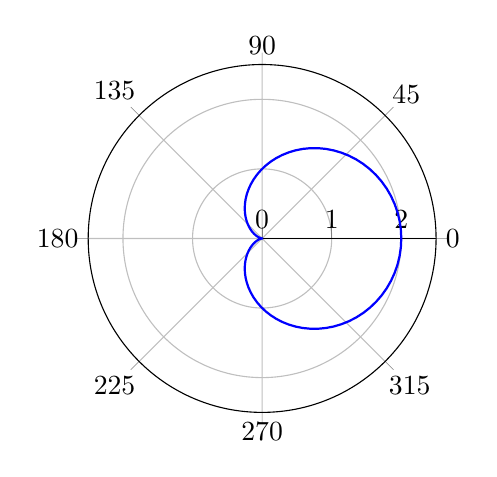
\begin{tikzpicture}
    \begin{polaraxis}[
        xlabel={}, ylabel={}, % 不显示坐标轴标签
        xmin=0, xmax=360, % 角度范围 0 到 360 度
        ymin=0, ymax=2.5, % r 的范围(根据 a 调整)
        width=6cm, height=6cm, % 图形大小
        samples=100, % 曲线平滑度
    ]
        \addplot[blue, thick, domain=0:360] {1 + cos(x)};
    \end{polaraxis}
\end{tikzpicture}
    \end{center}
    \begin{align*}
        S &=\int_{0}^{2\pi}\sqrt{a^2(1+\cos{\theta})^2+a^2\sin{\theta}^2}\d \theta \\
        &=\sqrt{2}a\int_{0}^{2\pi}\sqrt{1+\cos{\theta}}\d \theta \\
        &\xlongequal{\cos{\theta}=2\cos^2{\frac{\theta}{2}}-1}2a\int_{0}^{2\pi}\left|\cos\frac{\theta}{2}\right|\d\theta \\
        &=8a
    \end{align*}
    \end{solution}
\end{enumerate}

\section{ 定积分应用求侧面积}

\begin{enumerate}[label=\arabic*.,start=19]
    \item (2016,数二)设$D$是由曲线$y=\sqrt{1-x^2}(0\leq x\leq 1)$与
    $\begin{cases}
        x=\cos^3t \\
        y=\sin^3t 
    \end{cases}(0\leq t\leq \frac{\pi}{2})$围成的平面区域,求$D$绕$x$轴旋转一周所得旋转体的体积和表面积.
    
    \begin{solution}
    这个参数方程的图像是需要记住即星形线
    \begin{center}
        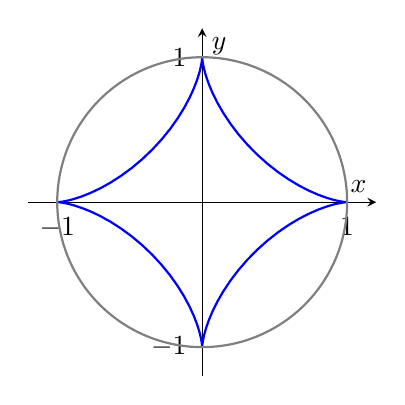
\begin{tikzpicture}
            \begin{axis}[
        axis lines=center,
        xlabel={$x$},
        ylabel={$y$},
        xmin=-1.2, xmax=1.2,
        ymin=-1.2, ymax=1.2,
        width=6cm, height=6cm,
        samples=100,
        domain=0:2*pi,
    ]
        \addplot[blue, thick] ({(cos(deg(x)))^3}, {(sin(deg(x)))^3});
        \addplot[domain=0:2*pi, samples=100, smooth, thick, gray] ({cos(deg(x))}, {sin(deg(x))});
            \end{axis}
        \end{tikzpicture}
    \end{center}
    \begin{align*}
        V &=\frac{1}{4}\cdot\frac{4}{3}\pi\cdot 1^3 - \int_{0}^{1}\pi y^2(x)\d x \\
        &=\frac{18}{35}\pi \\
        S &=\frac{1}{2}\cdot 4\pi + \int_{0}^{1}2\pi y(x)\d s \\
        &=2\pi + \int_{0}^{\frac{\pi}{2}}2\pi\cdot\sin^3{t}\sqrt{(3\cos^2{t}(-\sin{t}))^2+(3\sin^2{t}\cos{t})^2}\d t \\
        &=\frac{16\pi}{5}
    \end{align*}
    \end{solution}
\end{enumerate}

\section{证明含有积分的等式或不等式}
\begin{remark}
    积分中值定理(三个) \\
    (一) 第一积分中值定理,若$f(x)$在$[a,b]$上连续,则
    $$
    \exists c\in[a,b], \int_{a}^{b}f(x)\d x = f(c)(b-a)
    $$
    (二) 第一积分中值定理的推广,若$f(x)$在$(a,b)$上连续
    $$
    \exists c\in(a,b), \int_{a}^{b}f(x)\d x = f(c)(b-a)
    $$
    (三) 第二积分中值定理,若$f(x),g(x)$在区间$(a,b)$上连续,且$g(x)$在其上不变号则
    $$
    \exists c\in (a,b), \int_{a}^{b}f(x)g(x)\d x = g(c)\int_{a}^{b}f(x)\d x
    $$
    比较定理及其推论 \\
    设函数$f(x),g(x)$在$[a,b]$上可积,且$f(x)\leq g(x)$,则 $\int_{a}^{b}f(x)\leq \int_{a}^{b}g(x)$ \\
    推论一: 若函数$f(x),g(x)$在$[a,b]$ {\color{red} 连续},且$f(x)\leq g(x)$,则$\int_{a}^{b}f(x) < \int_{a}^{b}g(x)$ \\
    推论二: 若$f(x)\geq 0$,$x\in[a,b]$,则$\int_{a}^{b}f(x)\d x\geq 0$ \\
    推论三: $\left|\int_{a}^{b}f(x)\d x\right|\leq \int_{a}^{b}\left|f(x)\right|\d x$
\end{remark}

\newpage

\begin{enumerate}[label=\arabic*.,start=21]
    \item (2000,数二)设函数$S(x)=\int_0^x|\cos t| dt$.
    \begin{enumerate}[label=(\roman*)]
        \item[(1)] 当$n$为正整数,且$n\pi\leq x<(n+1)\pi$时,证明$2n\leq S(x)<2(n+1)$;
        \item[(2)] 求$\lim_{x\to+\infty}\frac{S(x)}{x}$
    \end{enumerate}
    
    \begin{solution}
    (1)由比较定理有
    $$
    \int_{0}^{n\pi}\left|\cos{t}\right|\d t \leq S(x) < \int_{0}^{(n+1)\pi}\left|\cos{t}\right|\d t
    $$
    显然$\left|\cos{t}\right|$以$\pi$为周期故上式容易计算为
    $$
    2n\leq S(x)<2(n+1)
    $$
    (2) 考虑夹逼准则
    $$
    \frac{2}{\pi}\xleftarrow{\lim_{n\to\infty}}\frac{2n}{(n+1)\pi} \leq \frac{S(x)}{x} < \frac{2(n+1)}{n\pi}\xrightarrow{\lim_{n\to\infty}}\frac{2}{\pi}
    $$
    故$\lim_{x\to\infty}\frac{S(x)}{x}=\frac{2}{\pi}$
    \end{solution}
    
    \item (2014,数二、数三)设函数$f(x), g(x)$在区间$[a, b]$上连续,且$f(x)$单调增加,$0\leq g(x)\leq 1$.
    证明:
    \begin{enumerate}[label=(\roman*)]
        \item[(1)] $0\leq\int_a^x g(t) dt\leq x-a, x\in[a, b]$;
        \item[(2)] $\int_a^{a+\int_a^b g(t) dt} f(x) dx\leq\int_a^b f(x) g(x) dx$.
    \end{enumerate}
    
    \begin{solution}
    (一)由比较定理有 
    $$
    0\leq \int_{a}^{x}g(x)\d x\leq \int_{a}^{x}\d x = x - a 
    $$
    (二) 构建函数用单调性 \\
    令
    $$
    F(x)=\int_{a}^{ma+\int_{a}^{x}g(t)\d t}f(t)\d t - \int_{a}^{x}f(t)g(t)\d t
    $$ 
    则其导数为
    $$
    F'(x)=g(x)\left[f(a+\int_{a}^{x}g(t)\d t)-f(x)\right] 
    $$
    由一可知 $a+\int_{a}^{x}g(t)\d t \leq x$ 
    从而可知$F'(x) < 0$ 故而$F(x)$在区间$(a,b)$上单调递减,而$F(a)=0$故$F(b)<F(a)=0$ 即
    $$
    \int_a^{a+\int_a^b g(t) dt} f(x) dx\leq\int_a^b f(x) g(x) dx
    $$.
    \end{solution}
\end{enumerate}

\ifx\allfiles\undefined
\end{document}
\fi